\documentclass[twoside]{article}

% Packages required by doxygen
\usepackage{fixltx2e}
\usepackage{calc}
\usepackage{doxygen}
\usepackage{graphicx}
\usepackage[utf8]{inputenc}
\usepackage{makeidx}
\usepackage{multicol}
\usepackage{multirow}
\PassOptionsToPackage{warn}{textcomp}
\usepackage{textcomp}
\usepackage[nointegrals]{wasysym}
\usepackage[table]{xcolor}

% Font selection
\usepackage[T1]{fontenc}
\usepackage{mathptmx}
\usepackage[scaled=.90]{helvet}
\usepackage{courier}
\usepackage{amssymb}
\usepackage{sectsty}
\renewcommand{\familydefault}{\sfdefault}
\allsectionsfont{%
  \fontseries{bc}\selectfont%
  \color{darkgray}%
}
\renewcommand{\DoxyLabelFont}{%
  \fontseries{bc}\selectfont%
  \color{darkgray}%
}
\newcommand{\+}{\discretionary{\mbox{\scriptsize$\hookleftarrow$}}{}{}}

% Page & text layout
\usepackage[screen]{geometry}
\tolerance=750
\hfuzz=15pt
\hbadness=750
\setlength{\emergencystretch}{15pt}
\setlength{\parindent}{0cm}
\setlength{\parskip}{0.2cm}
\makeatletter
\renewcommand{\paragraph}{%
  \@startsection{paragraph}{4}{0ex}{-1.0ex}{1.0ex}{%
    \normalfont\normalsize\bfseries\SS@parafont%
  }%
}
\renewcommand{\subparagraph}{%
  \@startsection{subparagraph}{5}{0ex}{-1.0ex}{1.0ex}{%
    \normalfont\normalsize\bfseries\SS@subparafont%
  }%
}
\makeatother

% Headers & footers
\usepackage{fancyhdr}
\pagestyle{fancyplain}
\fancyhead[LE]{\fancyplain{}{\bfseries\thepage}}
\fancyhead[CE]{\fancyplain{}{}}
\fancyhead[RE]{\fancyplain{}{\bfseries\leftmark}}
\fancyhead[LO]{\fancyplain{}{\bfseries\rightmark}}
\fancyhead[CO]{\fancyplain{}{}}
\fancyhead[RO]{\fancyplain{}{\bfseries\thepage}}
\fancyfoot[LE]{\fancyplain{}{}}
\fancyfoot[CE]{\fancyplain{}{}}
\fancyfoot[RE]{\fancyplain{}{\bfseries\scriptsize Generated on Tue Oct 17 2017 14\+:33\+:40 for Lab 4 Pizza by Doxygen }}
\fancyfoot[LO]{\fancyplain{}{\bfseries\scriptsize Generated on Tue Oct 17 2017 14\+:33\+:40 for Lab 4 Pizza by Doxygen }}
\fancyfoot[CO]{\fancyplain{}{}}
\fancyfoot[RO]{\fancyplain{}{}}
\renewcommand{\footrulewidth}{0.4pt}
\renewcommand{\sectionmark}[1]{%
  \markright{\thesection\ #1}%
}

% Indices & bibliography
\usepackage{natbib}
\usepackage[titles]{tocloft}
\setcounter{tocdepth}{3}
\setcounter{secnumdepth}{5}
\makeindex

% Packages requested by user
\usepackage{titlesec}

% Hyperlinks (required, but should be loaded last)
\usepackage{ifpdf}
\ifpdf
  \usepackage[pdftex,pagebackref=true]{hyperref}
\else
  \usepackage[ps2pdf,pagebackref=true]{hyperref}
\fi
\hypersetup{%
  colorlinks=true,%
  linkcolor=blue,%
  citecolor=blue,%
  unicode%
}

% Custom commands
\newcommand{\clearemptydoublepage}{%
  \newpage{\pagestyle{empty}\cleardoublepage}%
}


\newcommand{\sectionbreak}{\clearpage}

\begin{document}

% Titlepage & ToC
\hypersetup{pageanchor=false,
             bookmarks=true,
             bookmarksnumbered=true,
             pdfencoding=unicode
            }
\pagenumbering{roman}
\begin{titlepage}
\vspace*{7cm}
\begin{center}%
{\Large Lab 4 Pizza }\\
\vspace*{1cm}
{\large Generated by Doxygen 1.8.8}\\
\vspace*{0.5cm}
{\small Tue Oct 17 2017 14:33:40}\\
\end{center}
\end{titlepage}
\tableofcontents
\pagenumbering{arabic}
\hypersetup{pageanchor=true}

%--- Begin generated contents ---
\section{Specification}
\label{Specification}
\hypertarget{Specification}{}
This program has a built in dictionary for english that can be translated to tagalog. It has a user input in which the user may add the translation of a word that is not within the dictionary. 
\section{Analysis}
\label{Analysis}
\hypertarget{Analysis}{}
inputs will be\+:

\begin{DoxyItemize}
\item The outputs will be\+:\end{DoxyItemize}
\begin{DoxyItemize}
\item The overall algorithim is\+: \end{DoxyItemize}

\section{order\+\_\+cb}
\label{order_cb}
\hypertarget{order_cb}{}
This is the callback function to order a pizza


\begin{DoxyParams}{Parameters}
{\em void} & pointers not used \\
\hline
\end{DoxyParams}
\begin{DoxyReturn}{Returns}
void 
\end{DoxyReturn}

\section{File Index}
\subsection{File List}
Here is a list of all files with brief descriptions\+:\begin{DoxyCompactList}
\item\contentsline{section}{\hyperlink{BuildListDirectly_8cpp}{Build\+List\+Directly.\+cpp} }{\pageref{BuildListDirectly_8cpp}}{}
\item\contentsline{section}{\hyperlink{destroyList_8cpp}{destroy\+List.\+cpp} }{\pageref{destroyList_8cpp}}{}
\item\contentsline{section}{\hyperlink{displayList_8cpp}{display\+List.\+cpp} }{\pageref{displayList_8cpp}}{}
\item\contentsline{section}{\hyperlink{Insert_8cpp}{Insert.\+cpp} }{\pageref{Insert_8cpp}}{}
\item\contentsline{section}{\hyperlink{InsertInOrder_8cpp}{Insert\+In\+Order.\+cpp} }{\pageref{InsertInOrder_8cpp}}{}
\item\contentsline{section}{\hyperlink{lab2_8h}{lab2.\+h} }{\pageref{lab2_8h}}{}
\item\contentsline{section}{\hyperlink{loadList_8cpp}{load\+List.\+cpp} }{\pageref{loadList_8cpp}}{}
\item\contentsline{section}{\hyperlink{loadList2_8cpp}{load\+List2.\+cpp} }{\pageref{loadList2_8cpp}}{}
\item\contentsline{section}{\hyperlink{loadList3_8cpp}{load\+List3.\+cpp} }{\pageref{loadList3_8cpp}}{}
\item\contentsline{section}{\hyperlink{main_8cpp}{main.\+cpp} }{\pageref{main_8cpp}}{}
\end{DoxyCompactList}

\section{File Documentation}
\hypertarget{cook__cb_8cpp}{\subsection{cook\+\_\+cb.\+cpp File Reference}
\label{cook__cb_8cpp}\index{cook\+\_\+cb.\+cpp@{cook\+\_\+cb.\+cpp}}
}
{\ttfamily \#include \char`\"{}lab.\+h\char`\"{}}\\*
Include dependency graph for cook\+\_\+cb.\+cpp\+:\nopagebreak
\begin{figure}[H]
\begin{center}
\leavevmode
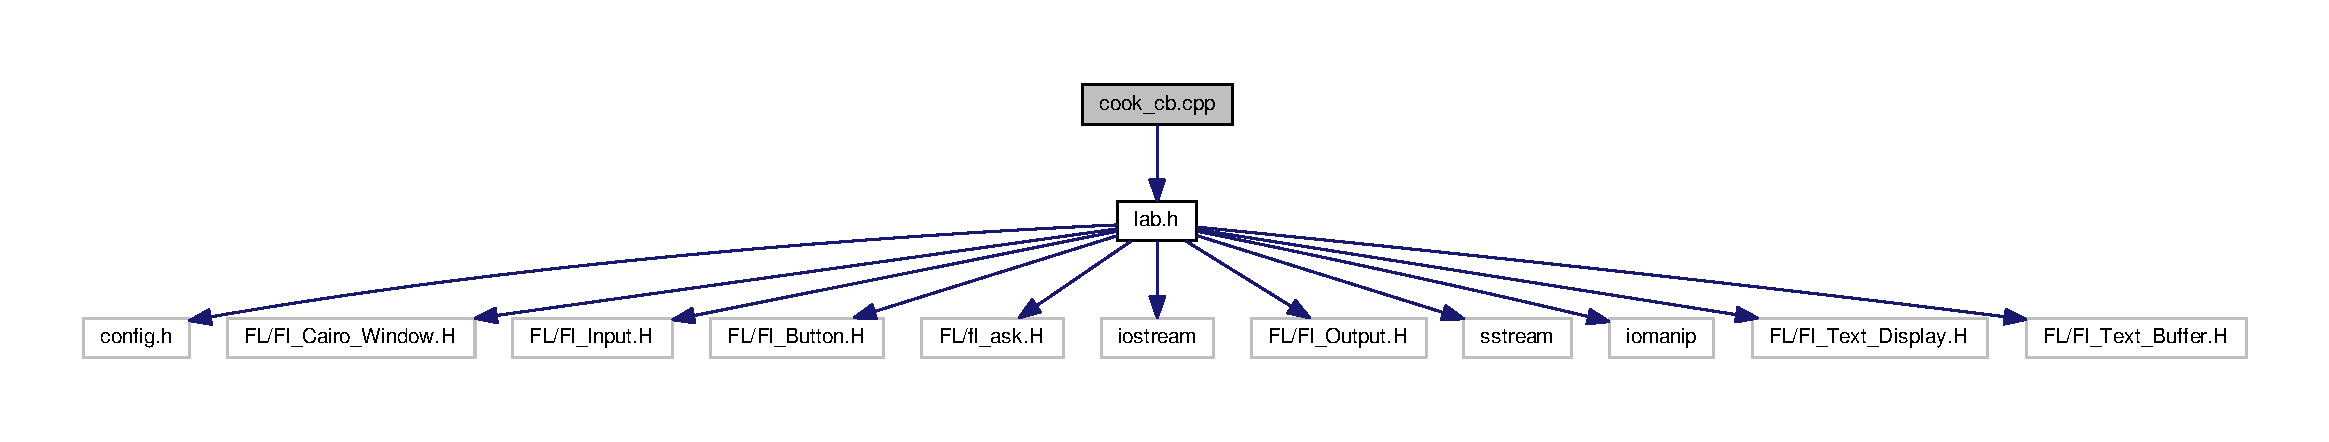
\includegraphics[width=350pt]{cook__cb_8cpp__incl}
\end{center}
\end{figure}
\subsubsection*{Functions}
\begin{DoxyCompactItemize}
\item 
void \hyperlink{cook__cb_8cpp_abb6fd11336b6e04e134b70abc225a8f6}{cook\+\_\+cb} (void $\ast$)
\end{DoxyCompactItemize}


\subsubsection{Function Documentation}
\hypertarget{cook__cb_8cpp_abb6fd11336b6e04e134b70abc225a8f6}{\index{cook\+\_\+cb.\+cpp@{cook\+\_\+cb.\+cpp}!cook\+\_\+cb@{cook\+\_\+cb}}
\index{cook\+\_\+cb@{cook\+\_\+cb}!cook\+\_\+cb.\+cpp@{cook\+\_\+cb.\+cpp}}
\paragraph[{cook\+\_\+cb}]{\setlength{\rightskip}{0pt plus 5cm}void cook\+\_\+cb (
\begin{DoxyParamCaption}
\item[{void $\ast$}]{}
\end{DoxyParamCaption}
)}}\label{cook__cb_8cpp_abb6fd11336b6e04e134b70abc225a8f6}

\begin{DoxyCode}
3 \{
4     \textcolor{comment}{//buff->text(pizza->value());}
5     
6     \textcolor{comment}{// temp solution, when it's cooked, put it}
7     \textcolor{comment}{// in the LLQueue; then here }
8     \textcolor{comment}{// use your new function that displays}
9     \textcolor{comment}{// what is in Q to create a string (with newlines)}
10     \textcolor{comment}{// in it, return it here and siplay that in the buffer}
11     
12 \}
\end{DoxyCode}

\hypertarget{lab_8dox}{\subsection{lab.\+dox File Reference}
\label{lab_8dox}\index{lab.\+dox@{lab.\+dox}}
}

\hypertarget{lab_8h}{\subsection{lab.\+h File Reference}
\label{lab_8h}\index{lab.\+h@{lab.\+h}}
}
{\ttfamily \#include \char`\"{}config.\+h\char`\"{}}\\*
{\ttfamily \#include $<$F\+L/\+Fl\+\_\+\+Cairo\+\_\+\+Window.\+H$>$}\\*
{\ttfamily \#include $<$F\+L/\+Fl\+\_\+\+Input.\+H$>$}\\*
{\ttfamily \#include $<$F\+L/\+Fl\+\_\+\+Button.\+H$>$}\\*
{\ttfamily \#include $<$F\+L/fl\+\_\+ask.\+H$>$}\\*
{\ttfamily \#include $<$iostream$>$}\\*
{\ttfamily \#include $<$F\+L/\+Fl\+\_\+\+Output.\+H$>$}\\*
{\ttfamily \#include $<$sstream$>$}\\*
{\ttfamily \#include $<$iomanip$>$}\\*
{\ttfamily \#include $<$F\+L/\+Fl\+\_\+\+Text\+\_\+\+Display.\+H$>$}\\*
{\ttfamily \#include $<$F\+L/\+Fl\+\_\+\+Text\+\_\+\+Buffer.\+H$>$}\\*
Include dependency graph for lab.\+h\+:\nopagebreak
\begin{figure}[H]
\begin{center}
\leavevmode
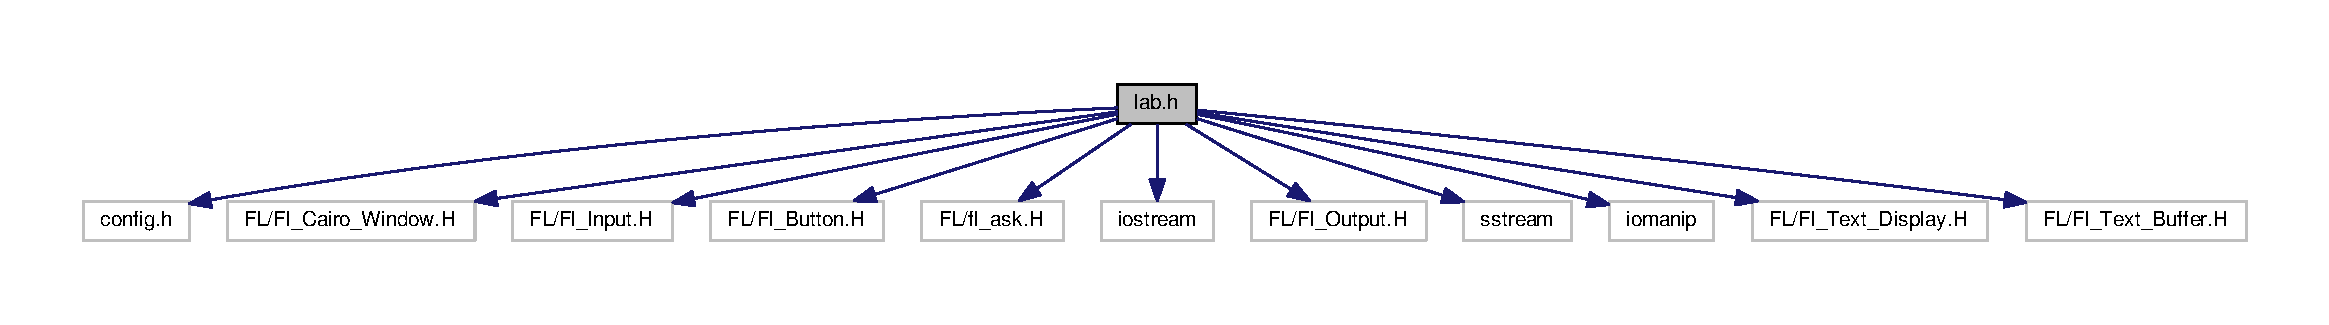
\includegraphics[width=350pt]{lab_8h__incl}
\end{center}
\end{figure}
This graph shows which files directly or indirectly include this file\+:\nopagebreak
\begin{figure}[H]
\begin{center}
\leavevmode
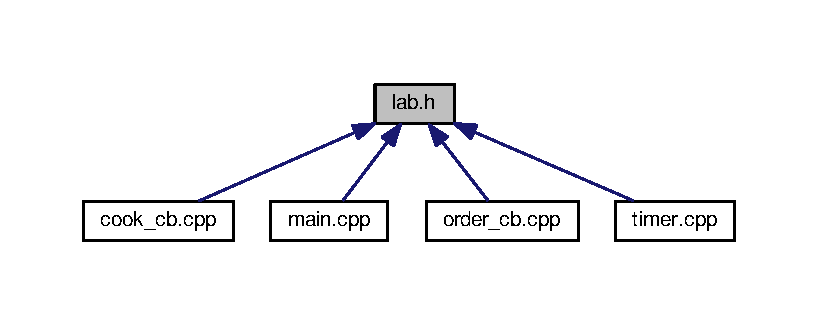
\includegraphics[width=350pt]{lab_8h__dep__incl}
\end{center}
\end{figure}
\subsubsection*{Functions}
\begin{DoxyCompactItemize}
\item 
void \hyperlink{lab_8h_a547f84331a8c529348e1130ca169c69c}{order\+\_\+cb} (void $\ast$, void $\ast$)
\item 
void \hyperlink{lab_8h_abb6fd11336b6e04e134b70abc225a8f6}{cook\+\_\+cb} (void $\ast$)
\item 
void \hyperlink{lab_8h_a13ed8751dfa95731ad8930762493b16b}{timer} (void $\ast$)
\end{DoxyCompactItemize}
\subsubsection*{Variables}
\begin{DoxyCompactItemize}
\item 
Fl\+\_\+\+Input $\ast$ \hyperlink{lab_8h_abf805c82a90897837d1c26ef915f1cd6}{pizza}
\item 
Fl\+\_\+\+Output $\ast$ \hyperlink{lab_8h_a05c7f6e86cca5f4d0ebf44d1f5042c37}{watch}
\item 
Fl\+\_\+\+Text\+\_\+\+Buffer $\ast$ \hyperlink{lab_8h_aea2b8efadc87a819fe57c311d668e504}{buff}
\item 
Fl\+\_\+\+Text\+\_\+\+Display $\ast$ \hyperlink{lab_8h_a23f917547a833922fd6bc8797cc04ee1}{order\+Q}
\end{DoxyCompactItemize}


\subsubsection{Function Documentation}
\hypertarget{lab_8h_abb6fd11336b6e04e134b70abc225a8f6}{\index{lab.\+h@{lab.\+h}!cook\+\_\+cb@{cook\+\_\+cb}}
\index{cook\+\_\+cb@{cook\+\_\+cb}!lab.\+h@{lab.\+h}}
\paragraph[{cook\+\_\+cb}]{\setlength{\rightskip}{0pt plus 5cm}void cook\+\_\+cb (
\begin{DoxyParamCaption}
\item[{void $\ast$}]{}
\end{DoxyParamCaption}
)}}\label{lab_8h_abb6fd11336b6e04e134b70abc225a8f6}

\begin{DoxyCode}
3 \{
4     \textcolor{comment}{//buff->text(pizza->value());}
5     
6     \textcolor{comment}{// temp solution, when it's cooked, put it}
7     \textcolor{comment}{// in the LLQueue; then here }
8     \textcolor{comment}{// use your new function that displays}
9     \textcolor{comment}{// what is in Q to create a string (with newlines)}
10     \textcolor{comment}{// in it, return it here and siplay that in the buffer}
11     
12 \}
\end{DoxyCode}
\hypertarget{lab_8h_a547f84331a8c529348e1130ca169c69c}{\index{lab.\+h@{lab.\+h}!order\+\_\+cb@{order\+\_\+cb}}
\index{order\+\_\+cb@{order\+\_\+cb}!lab.\+h@{lab.\+h}}
\paragraph[{order\+\_\+cb}]{\setlength{\rightskip}{0pt plus 5cm}void order\+\_\+cb (
\begin{DoxyParamCaption}
\item[{void $\ast$}]{, }
\item[{void $\ast$}]{}
\end{DoxyParamCaption}
)}}\label{lab_8h_a547f84331a8c529348e1130ca169c69c}

\begin{DoxyCode}
3 \{
4     fl\_alert(\hyperlink{lab_8h_abf805c82a90897837d1c26ef915f1cd6}{pizza}->value());
5     \textcolor{comment}{// cook it}
6     Fl::add\_timeout(5,\hyperlink{cook__cb_8cpp_abb6fd11336b6e04e134b70abc225a8f6}{cook\_cb});
7 \}
\end{DoxyCode}
\hypertarget{lab_8h_a13ed8751dfa95731ad8930762493b16b}{\index{lab.\+h@{lab.\+h}!timer@{timer}}
\index{timer@{timer}!lab.\+h@{lab.\+h}}
\paragraph[{timer}]{\setlength{\rightskip}{0pt plus 5cm}void timer (
\begin{DoxyParamCaption}
\item[{void $\ast$}]{}
\end{DoxyParamCaption}
)}}\label{lab_8h_a13ed8751dfa95731ad8930762493b16b}

\begin{DoxyCode}
3 \{
4     \textcolor{comment}{//std::cout << "1 sec" << std::endl;}
5     \textcolor{keyword}{static} \textcolor{keywordtype}{int} s= 0; \textcolor{keyword}{static} \textcolor{keywordtype}{int} m = 0;
6     std::ostringstream oss; \textcolor{comment}{// don't discard the memory. }
7                                               \textcolor{comment}{// keep it so we can update t to the window}
8     s++;    \textcolor{keywordflow}{if}(s == 59) \{s = 0; m++; \}
9     oss << std::setfill(\textcolor{charliteral}{'0'});
10     oss << std::setw(2) << m << \textcolor{stringliteral}{":"} << std::setw(2) << s;
11     \textcolor{comment}{//oss << s;}
12     \hyperlink{lab_8h_a05c7f6e86cca5f4d0ebf44d1f5042c37}{watch}->value(oss.str().c\_str());
13     
14     \textcolor{comment}{// Here we could check if the Q's have pizza and drivers}
15     \textcolor{comment}{// ready for delivery every 10 seconds so we can see order}
16     \textcolor{comment}{// in Q     if (s % 10 == 0)}
17     \textcolor{keyword}{static} std::string str;
18     std::string pizzas[] = \{\textcolor{stringliteral}{"veggie"},\textcolor{stringliteral}{"pepperoni"},\textcolor{stringliteral}{"sausage"},\textcolor{stringliteral}{"hawaiian"}\};
19     \textcolor{keywordflow}{if}(s % 10 == 0)
20     \{
21         str += pizzas[s%4] += \textcolor{stringliteral}{"\(\backslash\)n"};
22         \hyperlink{lab_8h_aea2b8efadc87a819fe57c311d668e504}{buff}->text(str.c\_str());
23     \}
24     
25     Fl::repeat\_timeout(1,\hyperlink{timer_8cpp_a13ed8751dfa95731ad8930762493b16b}{timer});
26 \}
\end{DoxyCode}


\subsubsection{Variable Documentation}
\hypertarget{lab_8h_aea2b8efadc87a819fe57c311d668e504}{\index{lab.\+h@{lab.\+h}!buff@{buff}}
\index{buff@{buff}!lab.\+h@{lab.\+h}}
\paragraph[{buff}]{\setlength{\rightskip}{0pt plus 5cm}Fl\+\_\+\+Text\+\_\+\+Buffer$\ast$ buff}}\label{lab_8h_aea2b8efadc87a819fe57c311d668e504}
\hypertarget{lab_8h_a23f917547a833922fd6bc8797cc04ee1}{\index{lab.\+h@{lab.\+h}!order\+Q@{order\+Q}}
\index{order\+Q@{order\+Q}!lab.\+h@{lab.\+h}}
\paragraph[{order\+Q}]{\setlength{\rightskip}{0pt plus 5cm}Fl\+\_\+\+Text\+\_\+\+Display$\ast$ order\+Q}}\label{lab_8h_a23f917547a833922fd6bc8797cc04ee1}
\hypertarget{lab_8h_abf805c82a90897837d1c26ef915f1cd6}{\index{lab.\+h@{lab.\+h}!pizza@{pizza}}
\index{pizza@{pizza}!lab.\+h@{lab.\+h}}
\paragraph[{pizza}]{\setlength{\rightskip}{0pt plus 5cm}Fl\+\_\+\+Input$\ast$ pizza}}\label{lab_8h_abf805c82a90897837d1c26ef915f1cd6}
\hypertarget{lab_8h_a05c7f6e86cca5f4d0ebf44d1f5042c37}{\index{lab.\+h@{lab.\+h}!watch@{watch}}
\index{watch@{watch}!lab.\+h@{lab.\+h}}
\paragraph[{watch}]{\setlength{\rightskip}{0pt plus 5cm}Fl\+\_\+\+Output$\ast$ watch}}\label{lab_8h_a05c7f6e86cca5f4d0ebf44d1f5042c37}

\hypertarget{main_8cpp}{\subsection{main.\+cpp File Reference}
\label{main_8cpp}\index{main.\+cpp@{main.\+cpp}}
}
{\ttfamily \#include \char`\"{}lab.\+h\char`\"{}}\\*
Include dependency graph for main.\+cpp\+:\nopagebreak
\begin{figure}[H]
\begin{center}
\leavevmode
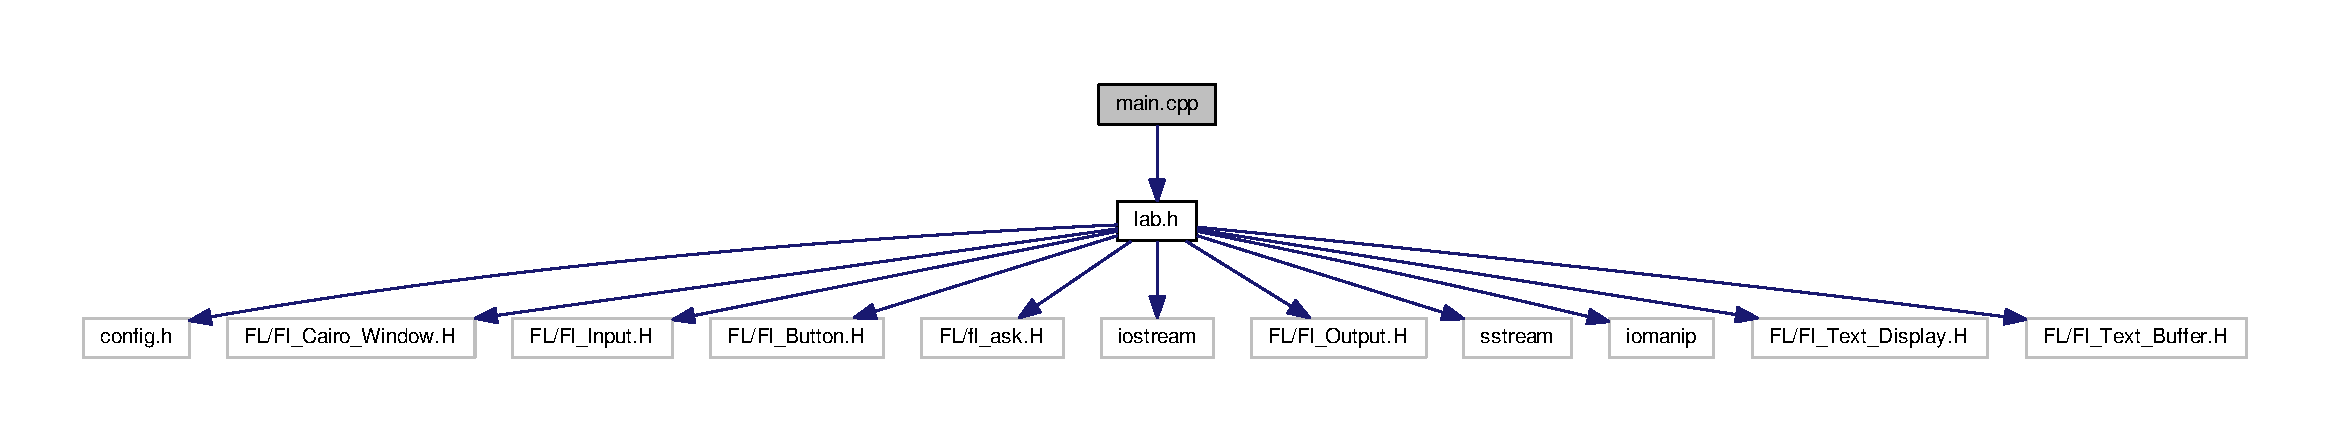
\includegraphics[width=350pt]{main_8cpp__incl}
\end{center}
\end{figure}
\subsubsection*{Functions}
\begin{DoxyCompactItemize}
\item 
int \hyperlink{main_8cpp_ae66f6b31b5ad750f1fe042a706a4e3d4}{main} ()
\end{DoxyCompactItemize}
\subsubsection*{Variables}
\begin{DoxyCompactItemize}
\item 
Fl\+\_\+\+Input $\ast$ \hyperlink{main_8cpp_abf805c82a90897837d1c26ef915f1cd6}{pizza}
\item 
Fl\+\_\+\+Output $\ast$ \hyperlink{main_8cpp_a05c7f6e86cca5f4d0ebf44d1f5042c37}{watch}
\item 
Fl\+\_\+\+Text\+\_\+\+Buffer $\ast$ \hyperlink{main_8cpp_aea2b8efadc87a819fe57c311d668e504}{buff}
\item 
Fl\+\_\+\+Text\+\_\+\+Display $\ast$ \hyperlink{main_8cpp_a23f917547a833922fd6bc8797cc04ee1}{order\+Q}
\end{DoxyCompactItemize}


\subsubsection{Function Documentation}
\hypertarget{main_8cpp_ae66f6b31b5ad750f1fe042a706a4e3d4}{\index{main.\+cpp@{main.\+cpp}!main@{main}}
\index{main@{main}!main.\+cpp@{main.\+cpp}}
\paragraph[{main}]{\setlength{\rightskip}{0pt plus 5cm}int main (
\begin{DoxyParamCaption}
{}
\end{DoxyParamCaption}
)}}\label{main_8cpp_ae66f6b31b5ad750f1fe042a706a4e3d4}

\begin{DoxyCode}
10 \{
11     Fl\_Cairo\_Window cw(400,300); \textcolor{comment}{// width & height of window}
12     cw.label(\textcolor{stringliteral}{"Pizza Deliveries Extravaganja"}); \textcolor{comment}{// title of your cairo window}
13     \textcolor{comment}{//cw.color(FL\_GREEN);}
14     
15     \hyperlink{main_8cpp_abf805c82a90897837d1c26ef915f1cd6}{pizza} = \textcolor{keyword}{new} Fl\_Input(190, 20, 100, 20, \textcolor{stringliteral}{"pizza:"});
16     \hyperlink{main_8cpp_abf805c82a90897837d1c26ef915f1cd6}{pizza}->labelcolor(FL\_BLUE);
17     
18     \hyperlink{main_8cpp_aea2b8efadc87a819fe57c311d668e504}{buff} = \textcolor{keyword}{new} Fl\_Text\_Buffer();
19     \hyperlink{main_8cpp_a23f917547a833922fd6bc8797cc04ee1}{orderQ} = \textcolor{keyword}{new} Fl\_Text\_Display(100,100,100,100,\textcolor{stringliteral}{"Order Q"});
20     \hyperlink{main_8cpp_a23f917547a833922fd6bc8797cc04ee1}{orderQ}->buffer(\hyperlink{main_8cpp_aea2b8efadc87a819fe57c311d668e504}{buff});
21     
22     \hyperlink{main_8cpp_a05c7f6e86cca5f4d0ebf44d1f5042c37}{watch} = \textcolor{keyword}{new} Fl\_Output(70,20,50,20,\textcolor{stringliteral}{"seconds:"});
23     
24     Fl\_Button b(330, 60, 50, 20, \textcolor{stringliteral}{"Order:"});
25     b.callback((Fl\_Callback*)\hyperlink{lab_8h_a547f84331a8c529348e1130ca169c69c}{order\_cb});
26     
27     cw.show();
28     Fl::add\_timeout(1,\hyperlink{lab_8h_a13ed8751dfa95731ad8930762493b16b}{timer});
29     \textcolor{keywordflow}{return} Fl::run();
30 \}
\end{DoxyCode}


\subsubsection{Variable Documentation}
\hypertarget{main_8cpp_aea2b8efadc87a819fe57c311d668e504}{\index{main.\+cpp@{main.\+cpp}!buff@{buff}}
\index{buff@{buff}!main.\+cpp@{main.\+cpp}}
\paragraph[{buff}]{\setlength{\rightskip}{0pt plus 5cm}Fl\+\_\+\+Text\+\_\+\+Buffer$\ast$ buff}}\label{main_8cpp_aea2b8efadc87a819fe57c311d668e504}
\hypertarget{main_8cpp_a23f917547a833922fd6bc8797cc04ee1}{\index{main.\+cpp@{main.\+cpp}!order\+Q@{order\+Q}}
\index{order\+Q@{order\+Q}!main.\+cpp@{main.\+cpp}}
\paragraph[{order\+Q}]{\setlength{\rightskip}{0pt plus 5cm}Fl\+\_\+\+Text\+\_\+\+Display$\ast$ order\+Q}}\label{main_8cpp_a23f917547a833922fd6bc8797cc04ee1}
\hypertarget{main_8cpp_abf805c82a90897837d1c26ef915f1cd6}{\index{main.\+cpp@{main.\+cpp}!pizza@{pizza}}
\index{pizza@{pizza}!main.\+cpp@{main.\+cpp}}
\paragraph[{pizza}]{\setlength{\rightskip}{0pt plus 5cm}Fl\+\_\+\+Input$\ast$ pizza}}\label{main_8cpp_abf805c82a90897837d1c26ef915f1cd6}
\hypertarget{main_8cpp_a05c7f6e86cca5f4d0ebf44d1f5042c37}{\index{main.\+cpp@{main.\+cpp}!watch@{watch}}
\index{watch@{watch}!main.\+cpp@{main.\+cpp}}
\paragraph[{watch}]{\setlength{\rightskip}{0pt plus 5cm}Fl\+\_\+\+Output$\ast$ watch}}\label{main_8cpp_a05c7f6e86cca5f4d0ebf44d1f5042c37}

\hypertarget{order__cb_8cpp}{\subsection{order\+\_\+cb.\+cpp File Reference}
\label{order__cb_8cpp}\index{order\+\_\+cb.\+cpp@{order\+\_\+cb.\+cpp}}
}
{\ttfamily \#include \char`\"{}lab.\+h\char`\"{}}\\*
Include dependency graph for order\+\_\+cb.\+cpp\+:\nopagebreak
\begin{figure}[H]
\begin{center}
\leavevmode
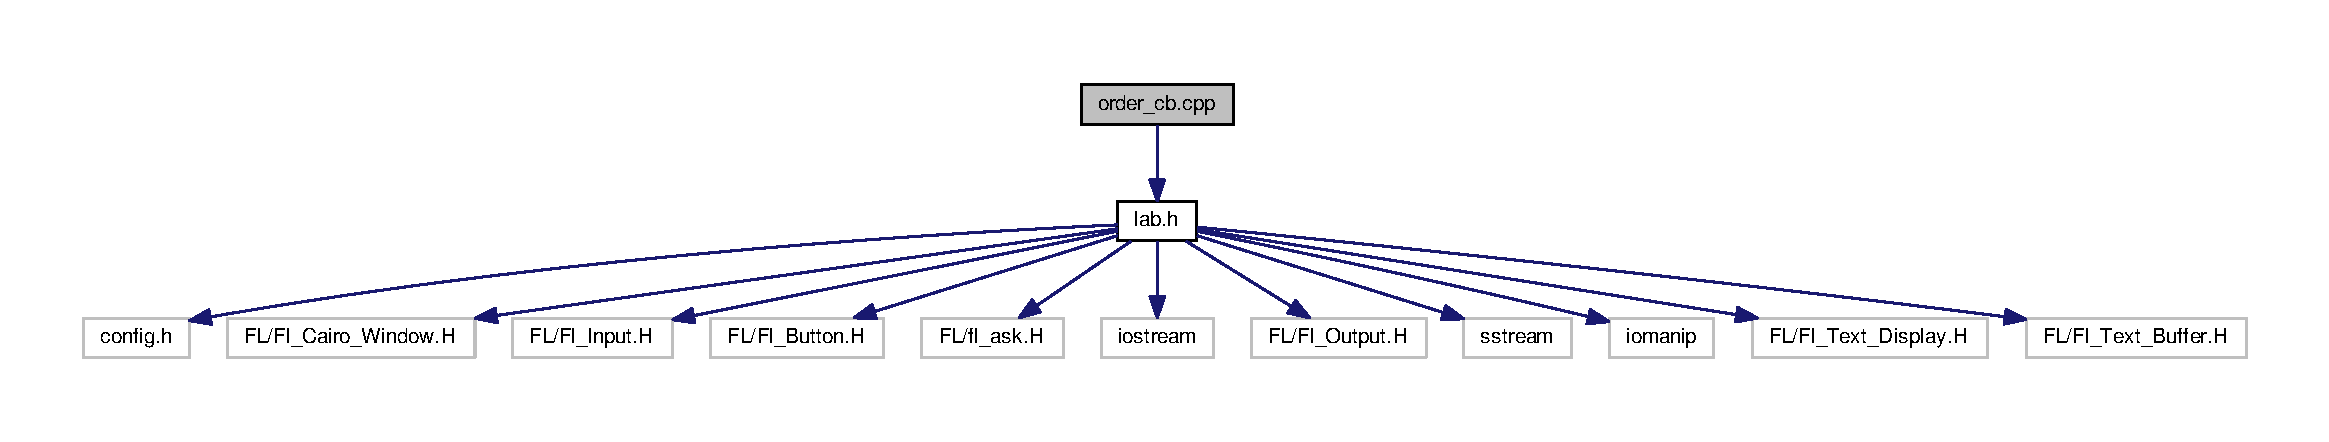
\includegraphics[width=350pt]{order__cb_8cpp__incl}
\end{center}
\end{figure}
\subsubsection*{Functions}
\begin{DoxyCompactItemize}
\item 
void \hyperlink{order__cb_8cpp_a547f84331a8c529348e1130ca169c69c}{order\+\_\+cb} (void $\ast$, void $\ast$)
\end{DoxyCompactItemize}


\subsubsection{Function Documentation}
\hypertarget{order__cb_8cpp_a547f84331a8c529348e1130ca169c69c}{\index{order\+\_\+cb.\+cpp@{order\+\_\+cb.\+cpp}!order\+\_\+cb@{order\+\_\+cb}}
\index{order\+\_\+cb@{order\+\_\+cb}!order\+\_\+cb.\+cpp@{order\+\_\+cb.\+cpp}}
\paragraph[{order\+\_\+cb}]{\setlength{\rightskip}{0pt plus 5cm}void order\+\_\+cb (
\begin{DoxyParamCaption}
\item[{void $\ast$}]{, }
\item[{void $\ast$}]{}
\end{DoxyParamCaption}
)}}\label{order__cb_8cpp_a547f84331a8c529348e1130ca169c69c}

\begin{DoxyCode}
3 \{
4     fl\_alert(\hyperlink{lab_8h_abf805c82a90897837d1c26ef915f1cd6}{pizza}->value());
5     \textcolor{comment}{// cook it}
6     Fl::add\_timeout(5,\hyperlink{cook__cb_8cpp_abb6fd11336b6e04e134b70abc225a8f6}{cook\_cb});
7 \}
\end{DoxyCode}

\hypertarget{timer_8cpp}{\subsection{timer.\+cpp File Reference}
\label{timer_8cpp}\index{timer.\+cpp@{timer.\+cpp}}
}
{\ttfamily \#include \char`\"{}lab.\+h\char`\"{}}\\*
Include dependency graph for timer.\+cpp\+:\nopagebreak
\begin{figure}[H]
\begin{center}
\leavevmode
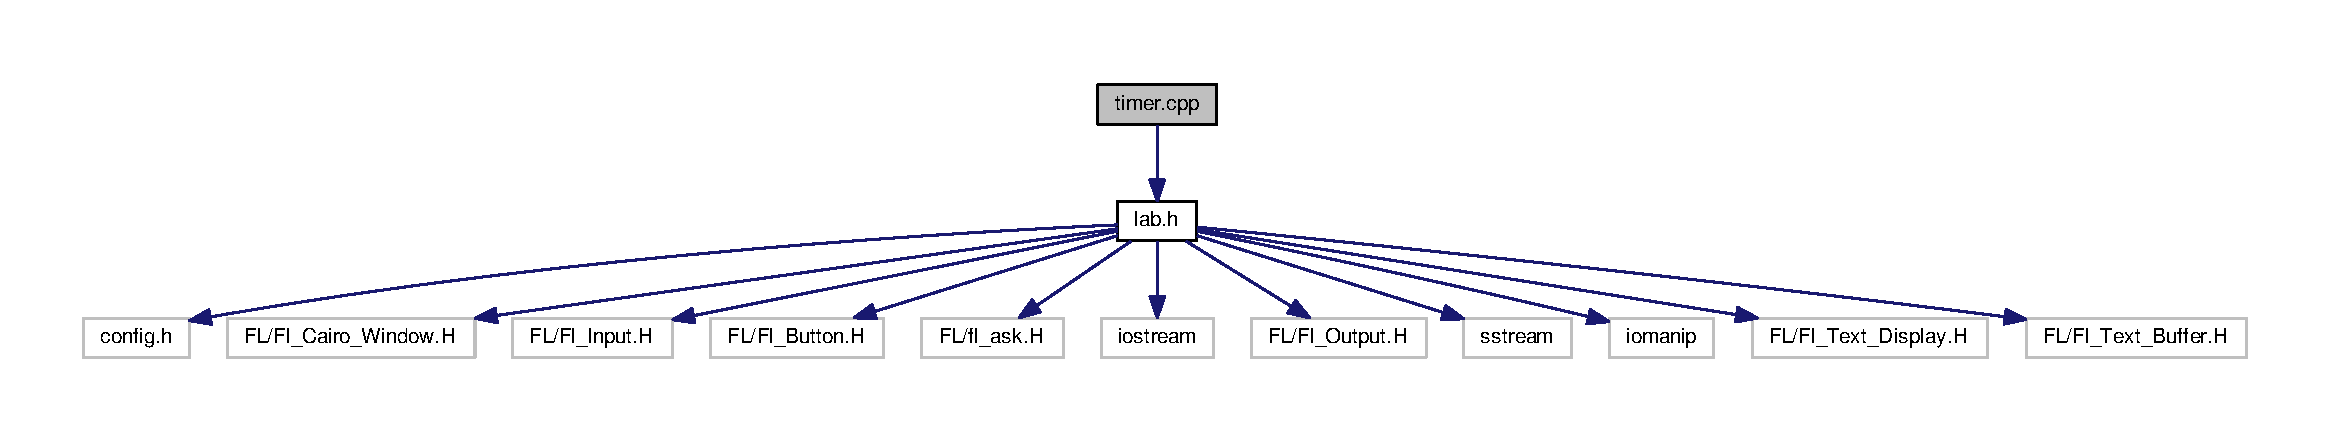
\includegraphics[width=350pt]{timer_8cpp__incl}
\end{center}
\end{figure}
\subsubsection*{Functions}
\begin{DoxyCompactItemize}
\item 
void \hyperlink{timer_8cpp_a13ed8751dfa95731ad8930762493b16b}{timer} (void $\ast$)
\end{DoxyCompactItemize}


\subsubsection{Function Documentation}
\hypertarget{timer_8cpp_a13ed8751dfa95731ad8930762493b16b}{\index{timer.\+cpp@{timer.\+cpp}!timer@{timer}}
\index{timer@{timer}!timer.\+cpp@{timer.\+cpp}}
\paragraph[{timer}]{\setlength{\rightskip}{0pt plus 5cm}void timer (
\begin{DoxyParamCaption}
\item[{void $\ast$}]{}
\end{DoxyParamCaption}
)}}\label{timer_8cpp_a13ed8751dfa95731ad8930762493b16b}

\begin{DoxyCode}
3 \{
4     \textcolor{comment}{//std::cout << "1 sec" << std::endl;}
5     \textcolor{keyword}{static} \textcolor{keywordtype}{int} s= 0; \textcolor{keyword}{static} \textcolor{keywordtype}{int} m = 0;
6     std::ostringstream oss; \textcolor{comment}{// don't discard the memory. }
7                                               \textcolor{comment}{// keep it so we can update t to the window}
8     s++;    \textcolor{keywordflow}{if}(s == 59) \{s = 0; m++; \}
9     oss << std::setfill(\textcolor{charliteral}{'0'});
10     oss << std::setw(2) << m << \textcolor{stringliteral}{":"} << std::setw(2) << s;
11     \textcolor{comment}{//oss << s;}
12     \hyperlink{lab_8h_a05c7f6e86cca5f4d0ebf44d1f5042c37}{watch}->value(oss.str().c\_str());
13     
14     \textcolor{comment}{// Here we could check if the Q's have pizza and drivers}
15     \textcolor{comment}{// ready for delivery every 10 seconds so we can see order}
16     \textcolor{comment}{// in Q     if (s % 10 == 0)}
17     \textcolor{keyword}{static} std::string str;
18     std::string pizzas[] = \{\textcolor{stringliteral}{"veggie"},\textcolor{stringliteral}{"pepperoni"},\textcolor{stringliteral}{"sausage"},\textcolor{stringliteral}{"hawaiian"}\};
19     \textcolor{keywordflow}{if}(s % 10 == 0)
20     \{
21         str += pizzas[s%4] += \textcolor{stringliteral}{"\(\backslash\)n"};
22         \hyperlink{lab_8h_aea2b8efadc87a819fe57c311d668e504}{buff}->text(str.c\_str());
23     \}
24     
25     Fl::repeat\_timeout(1,\hyperlink{timer_8cpp_a13ed8751dfa95731ad8930762493b16b}{timer});
26 \}
\end{DoxyCode}

%--- End generated contents ---

% Index
\newpage
\phantomsection
\addcontentsline{toc}{section}{Index}
\printindex

\end{document}
